
% \section*{Why $S^1$ is a double cover of the Mobius strip.}
% \newpage
\section{Galois covers}
\label{sec:GaloisCovers}

We  will assume that all our maps are simplicial and all our group actions are via simplicial maps.
For a space $X$, denote by $X_0$, $X_1$, $X_2$ the vertices, edges, and faces of $X$.
All our spaces are connected and locally finite.

We can construct covering maps using group actions.
A left group action of a group  $G$ on a space $Y$, denoted $G \groupaction Y$, is a collection of simplicial maps
\begin{align*}
  g \cdot (-) : Y &\longrightarrow Y
\end{align*}
for $g \in G$ satisfying
\begin{enumerate}
  \item ${\mathbb{1}} \cdot (-) = \id$,
  \item $g \cdot (h \cdot (-)) = (gh) \cdot (-)$.
\end{enumerate}
\begin{qbox}
  Show that a group always acts via isomorphisms i.e. $g \cdot (-) : Y \rightarrow Y$ is an isomorphism.
\end{qbox}

\begin{definition}
  We say that the action of $G$ on $Y$ is \emph{free} if the induced group action on sets $Y_0$, $Y_1$, and $Y_2$ is free.
  The \emph{quotient space} $Y/G$ is the space with vertices, edges, and faces given by $Y_0/G$, $Y_1/G$, and $Y_2/G$ respectively.
\end{definition}

\begin{ex}
  If $d | n$ then the cyclic group $\bbz/d$ acts freely on $nS^1$ and the quotient space is precisely $(n/d)S^1$.
\end{ex}

\begin{qbox}
  Check that if $G \groupaction Y$ is free then $Y \rightarrow Y/G$ is a cover.\tablefootnote{For groups acting via continuous maps (and not simplicial maps) it is not true that $Y \rightarrow Y / G$ is always a covering space. We further require the group action to be \emph{properly discontinuous}. Fortunately, a group action via simplicial maps is always properly discontinuous.}
\end{qbox}
\begin{definition}
  We say that a cover $p:Y \rightarrow X$ is \emph{Galois} if there exists a left group action $G \groupaction Y$ such that $X \cong Y/G$.
\end{definition}
This definition is less that ideal as it relies on the existence of an abstract group $G$.
We will find an equivalent criterion for $p:Y \rightarrow X$ to be Galois which is completely intrinsic to the cover $p$.











\subsection{Paths and covers}
For the rest of Section \ref{sec:GaloisCovers}, fix a connected cover $p: Y \longrightarrow X$.

\begin{definition}
  For a vertex $x$ in $X$, $p^{-1}(x)$ is the \emph{fiber} over $x$.
\end{definition}



A \emph{path} of length $k$ in $X$ is a finite sequence of edges $\gamma = e_1 e_2 \dots e_k$, where we allow inverses, such that $d_1 e_i = d_0 e_{i+1}$ for $1 \le i \le k-1$.
Define $d_0 \gamma = d_0 e_1$ and $d_1 \gamma = d_1 e_k$.
Denote by $\gamma^{-1}$ the reverse path $e_k^{-1} \dots e_2^{-1} e_1^{-1}$.
% Two paths $\gamma_1, \gamma_2$ with $d_1 \gamma_1 = d_0 \gamma_2$ can be concatenated to get a path $\gamma_1 \cdot \gamma_2$ from $d_0 \gamma_1$ to $d_1 \gamma_2$.
% For $x \in X$, we'll denote by $\mathbb{1}_x$ the ``path of length 0'' at $x$.


  \begin{theorem}[Unique lifting of paths]
    \label{theorem:uniqueLiftingPaths}
    For every vertex $x$ in $X$, every path $\gamma$ in $X$ starting at $x$, and every vertex $y$ in the fiber $p^{-1}(x)$, there exists a unique path $\widetilde{\gamma}$ in $Y$ such that
    \begin{align*}
      \widetilde{\gamma} & \mbox{ starts at } y, \\
      p (\widetilde{\gamma}) &= \gamma.
    \end{align*}
    $\widetilde{\gamma}$ is called a \emph{lift} of $\gamma$.
  \end{theorem}

  \begin{qbox}
    Pick a path $\gamma$ of length 5 in $S^1 \vee S^1$.
    Draw lifts of $\gamma$ starting at the three different vertices in cover $(10)$ in Figure \ref{fig:CoveringsOfS1S1}.
  \end{qbox}

  \begin{proof}[Proof of Theorem \ref{theorem:uniqueLiftingPaths}]
    Proof is by induction on the length of $\gamma$.

    \emph{Base case: length of $\gamma = 1$.}
    Let $\gamma = e$ with $d_0 e = x$.
    Because $p$ is a covering map, there is a neighborhood of $x$ that is evenly covered. Hence, there is a unique edge (possibly an inverse) $\widetilde{e}$ with $d_0 \widetilde{e} = y$ and $p(\widetilde{e}) = e$. Then $\widetilde{\gamma} = \widetilde{e}$ is the required lift.
    \begin{qbox}
      Complete the induction step.
    \end{qbox}
  \end{proof}

    \begin{corollary}
      \label{corollary:surjectivityOfCovers}
      $p:Y \rightarrow X$ is surjective.
    \end{corollary}
    \begin{qbox}
      Prove that $p:Y_0 \rightarrow X_0$ is surjective by lifting appropriate paths. (Optional: Extend this proof to edges and faces.)
    \end{qbox}
    \begin{corollary}
      \label{corollary:cardinalityOfFibers}
      Every path $\gamma$ from $x_0$ to $x_1$ in $X$ naturally defines a bijection
      \begin{align*}
        p^{-1}(x_0) \longrightarrow p^{-1}(x_1).
      \end{align*}
      Hence, the fibers over any two vertices $x_0$, $x_1 \in X_0$, have the same cardinality.
    \end{corollary}
    \begin{qbox}
      Prove Corollary \ref{corollary:cardinalityOfFibers} using the lift of an appropriate path and it's inverse.
    \end{qbox}













\subsection{Deck transformations}
% Our goal is to come up with a criterion for $p$ being Galois.
% There is a very intricate relation between covering spaces and paths in the base space.




\begin{definition}
  A \emph{deck transformation} of $p$ is a simplicial map $\varphi: X \rightarrow X$ that commutes with $p$ i.e. $p = p \circ \varphi$.
  \begin{equation*}
    \begin{tikzcd}
      Y \ar[rr, "\varphi"] \ar[rd, "p"'] & & Y \ar[ld,"p"] \\
      & X
    \end{tikzcd}
  \end{equation*}
\end{definition}

\begin{qbox}
  Show that deck transformations of $p$ form a group.
\end{qbox}
Let $\Gal(Y|X)$ denote the group of deck transformations of $p: Y \rightarrow X$.
There is a natural left action of the group $\Gal(Y|X)$ on the space $Y$.

\begin{ex}
  For example, the Galois groups of the covers $(1)$, $(3)$, $(5)$ of $S^1 \vee S^1$ in Figure \ref{fig:CoveringsOfS1S1} are $\bbz/2$, $\set{\mathbb{1}}$, $\bbz/3$ respectively.
\end{ex}


\begin{qbox}
  Find the group of deck transformations of the covers $(2)$, $(6)$, $(7)$, $(8)$, $(9)$, $(10)$, $(11)$ of $S^1 \vee S^1$ in Figure \ref{fig:CoveringsOfS1S1}.
  For each of these covers $Y$, find quotient $Y / G$ where $G=\Gal(Y| S^1 \vee S^1)$.
\end{qbox}

\begin{qbox}
  Prov that for any vertex $x \in X$ and every deck transformation $\varphi \in \Gal(Y|X)$, we have $\varphi(p^{-1}(x)) = p^{-1}(x)$.
  Hence, the deck transformations permute the fibers over $x$.\tablefootnote{
  One can think of this as shuffling a deck of cards, hence the name ``deck'' transformations.}
\end{qbox}

% \begin{ex}
%   If $G \groupaction X$ freely then every element $ g \in G$ defines a decktransformation of $p: X \rightarrow G \backslash X$.
% \end{ex}

\begin{theorem}
  \label{theorem:freenessGaloisAction}
  The action of $\Gal(Y|X)$ on $Y$ is free.
\end{theorem}
\begin{proof}
  We will show that if a deck transformation $\varphi \in \Gal(Y|X)$ does not act freely on $ Y$, then $\varphi$ fixes everything and hence is the identity element in $\Gal(Y|X)$.

  Suppose the action of $\varphi$ is not free. It suffices to assume that $g$ fixes some vertex, as if $\varphi$ fixes some edge or a face then it also fixes the vertices of the edge or the face respectively. Suppose $\varphi y_0 = y_0$ for $y_0 \in Y$.

  Consider another vertex $y$ in $Y$. Let $x_0 = p(y_0)$ and $x = p(y)$.
  \begin{qbox}
    Using a path $\gamma$ in $Y$ from $y_0$ to $y$ show that $\varphi$ fixes $y$, thereby completing the proof of the proposition.
  \end{qbox}
\end{proof}


\begin{corollary}
  \label{cor:deckTransforms}
  Let $y$ be a vertex in $Y$ and let $\varphi, \varphi' \in \Gal(Y|X)$ be two deck transformations. If $\varphi(y) = \varphi'(y)$ then $\varphi = \varphi'$. Hence, a deck transformation is completely determined by where it sends one vertex!
\end{corollary}
\begin{qbox}
  Prove this.\hint{Look at $\varphi^{-1} \circ \varphi'$.}
\end{qbox}

\begin{theorem}
  \label{theorem:GaloisCriterion}
  A cover $p:Y \rightarrow X$ is Galois if and only if $\Gal(Y|X)$ acts freely, transitively on each of the sets $p^{-1}(x)$ where $x$ is a vertex, an edge, or a face in $X$.
\end{theorem}
\begin{proof}
  This is equivalent to showing that $p:Y \rightarrow X$ is Galois if and only if for any two $y_1$, $y_2 \in p^{-1}(x)$ there is a unique deck transformation $g \in \Gal(Y|X)$ such that $g \cdot y_1 = y_2$.

  $(\Leftarrow)$ As $\Gal(Y|X)$ acts freely on $Y$, we can form the quotient $Y / \Gal(Y|X)$. Because the action is transitive, $X$ is isomorphic to $Y/G$.
  This proves one direction.

  $(\Rightarrow)$ Suppose $p$ is Galois and $X = Y/G$. We will show that the group of deck transformations of $p: Y \rightarrow Y/G$ is precisely $G$.
  Let $y$ be a vertex in $Y$ and let $x = p(y)$ be a vertex in $X$.
  By definition, The elements of $G$ act freely, transitively on the fiber $p^{-1}(x)$.
  By Corollary \ref{cor:deckTransforms} there can be no other deck transformations.
  Hence, $\Gal(Y|X) = G$.
  This proves the other direction.
\end{proof}

\begin{qbox}
  Which of the covers in Figure \ref{fig:CoveringsOfS1S1} are Galois?
\end{qbox}
\begin{qbox}
  Show that the 2-covers
  \begin{align*}
    \mbox{Cylinder} &\longrightarrow \mbox{Mobius Strip} \\
    \mbox{Torus} &\longrightarrow \mbox{Klein Bottle} \\
    \mbox{Sphere } S^2 &\longrightarrow \mbox{Real projective space}
  \end{align*}
  are all Galois.
\end{qbox}

Galois covers are completely symmetric covers.
By the evenly covered property of a covering space, small. neighborhoods of points in the fiber $p^{-1}(x)$ look the same as neighborhoods of $x$.
But in a Galois cover, the entire space $Y$ looks the same ``as seen from any point in the fiber''.
In general, an oject being Galois means that it is as symmetric as possible.


\begin{remark}
  The analogy with field theory is very clear here.
  We study field extensions $E \rightarrow F$ in the Galois extensions of fields.
  The deck transformations are replaced by automorphisms of $F$ which fix $E$, group quotients are replaced by fixed points.
  An extension is Galois precisely when $F^{\Gal(E|F)} = E$.
\end{remark}






\begin{figure}[p]
\centering
  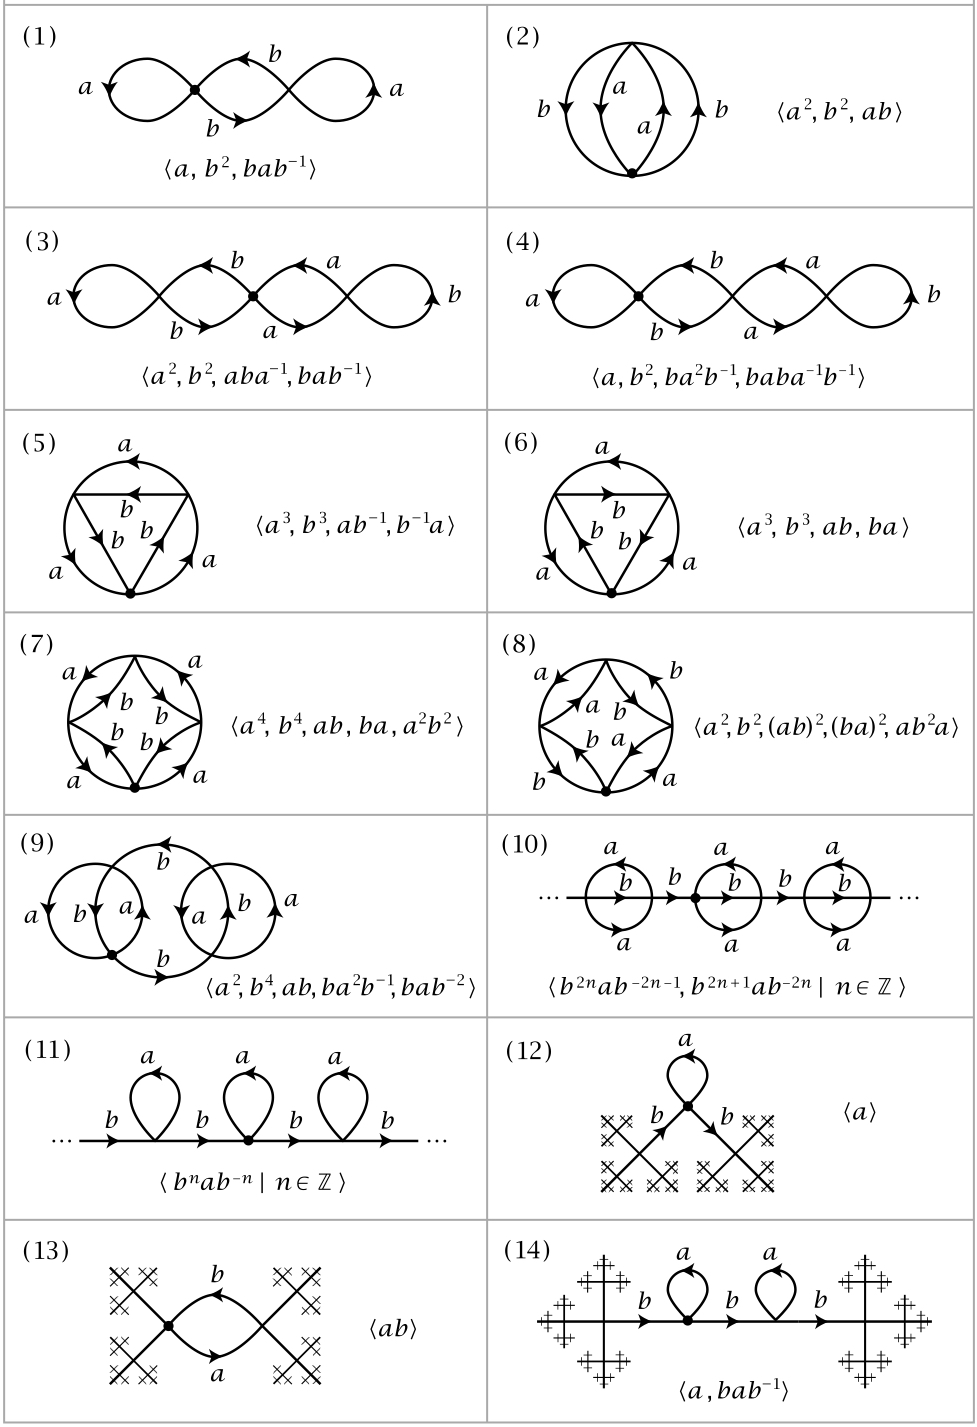
\includegraphics[width=\textwidth]{coveringsOfS1S1.jpg}
  \caption*{Coverings of $S^1 \vee S^1$. Image from Algebraic Topology, Allen Hatcher, Chapter 1.}
  % \label{fig:CoveringsOfS1S1}
\end{figure}
